\section{Results}
\label{sec:results}

Through this section we discuss the experimental tests, along with the valuation 
strategy carried out. 

The main purpose of our test is to understand how many tags for each service are 
correctly addressed. In order to achieve this, we distributed GHio-Ca to some 
testers and asked to deselect tags that did not concern shots that they have 
taken. Finally, they had to send the result to us.

Our approach was to make as simple as possible for the tester to contribute: we 
(i) made a video tutorial\footnote{\url{https://youtu.be/G9PSzpBI5LA}} in which 
we showed what they had to do, (ii) wrote a mini-wiki where the experiment was 
explained, (iii) modified the application. 

According to our planning, to each testing member was asked to take 5 photos. 
The final number of photos that we received is 150.

\subsection{Tester vs Normal version}

We needed to implement three main changes to the normal version to be able to 
carry on the experiment. The first one is about the way we retrieved results 
from services: in the normal version, the tags are merged together, instead in 
the test version we did not merge them.
Abuse of APIs calls from users was our main concern. To solve this issue, we put 
a limit on the maximum number of pictures that a tester could take.
Last but not least is how the results are shared. With the test version, we only 
allowed users to share the content with e-mail applications, sending tags and 
photos to our email address.


\subsection{Graphical analysis}

At the end of the testing phase, we collected all the e-mails received, we 
counted them and, exploiting \texttt{R}, we built several graphical 
rappresentations that we explain as follows.

\begin{figure}[H]
\centering
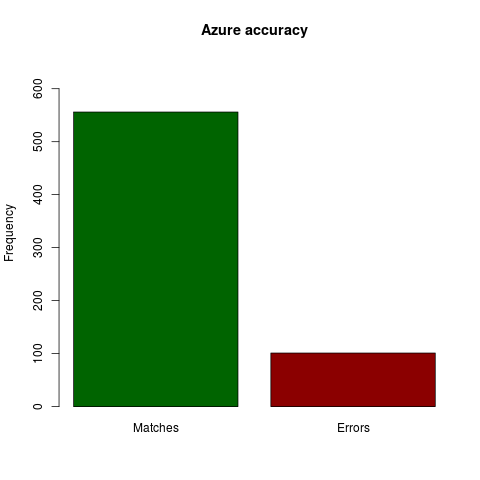
\includegraphics[scale=0.4]{AzureGraph}
\caption{Histogram of Azure tagging results (679 tags provided, 574 matches, 105 
mismatch)}
\label{img:testgraphsazure}
\end{figure}

As we can see in Figure~\ref{img:testgraphsazure}, Azure behaviour is pretty 
good, with 85\% circa of correct tags. This is the best result we are able to 
obtain.

\begin{figure}[H]
\centering
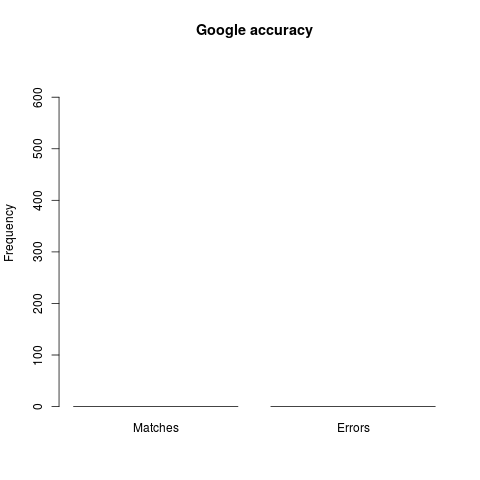
\includegraphics[scale=0.4]{GoogleGraph}
\caption{Histogram of Google tagging results (32 tags provided, 10 matches, 22 
mismatch)}
\label{img:testgraphgoogle}
\end{figure}

As we can see in Figure~\ref{img:testgraphgoogle}, using Google Image search, we 
obtained the worst performance among the services we used. Rarely we had tags 
from this service, with 32 tags only 10 were correct, with a 31\% of correct 
tags. As a matter of fact, Google Image search was not designed to provide tags 
from/to user images, thus we did not expect good results from this service.

\begin{figure}[H]
\centering
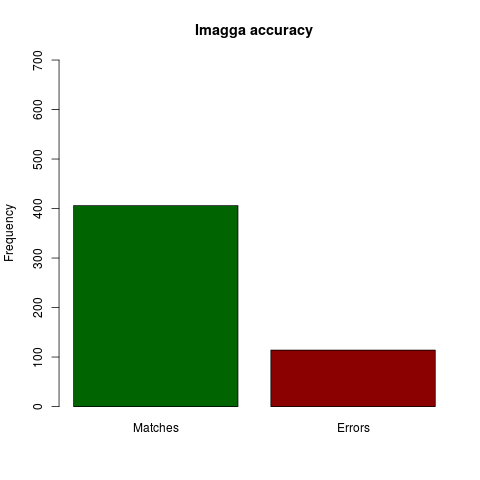
\includegraphics[scale=0.4]{ImaggaGraph}
\caption{Histogram of Imagga tagging results (507 tags provided, 394 matches, 
113 mismatch)}
\label{img:testgraphimagga}
\end{figure}

Imagga is an minor service that we discovered searching online. This provider 
give us 78\% of correct tags (Figure~\ref{img:testgraphimagga}). It is important 
to keep in mind that most of the bad tags were filtered by our application 
before getting displayed to the user. We displayed tags with more than 0.7 of 
confidence.

\begin{figure}[H]
\centering
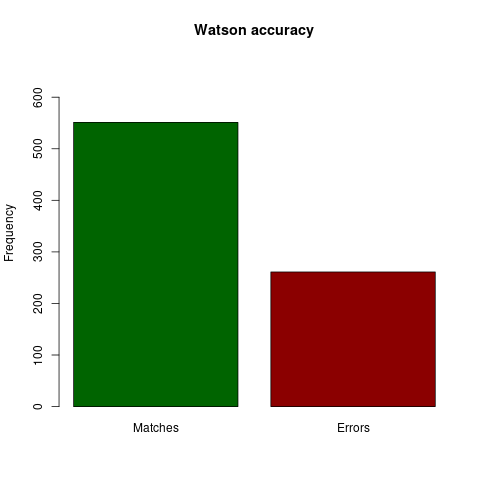
\includegraphics[scale=0.4]{WatsonGraph}
\caption{Histogram of Watson tagging results (812 tags provided, 551 matches, 
261 mismatch)}
\label{img:testgraphwatson}
\end{figure}

Watson is an IBM service for image recognition. From the results we observed 
that the service provided a lot of tags, but a good chunk were wrong, with only 
68\% of correct one (Figure~\ref{img:testgraphwatson}).

\begin{figure}[H]
\centering
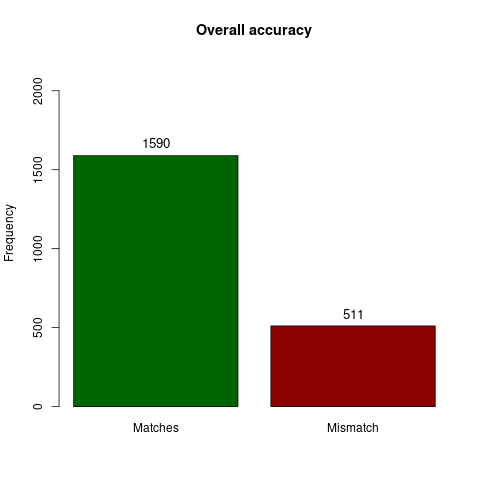
\includegraphics[scale=0.4]{OverallGraph}
\caption{Histogram of all tagging results (2030 tags provided, 1529 matches, 501 
mismatch)}
\label{img:testgraphoverall}
\end{figure}

In Figure~\ref{img:testgraphoverall} we can see the overall representation, with 
a percentage of 75\% of correct tags, that we consider it to be a good result.

\begin{figure}[H]
\centering
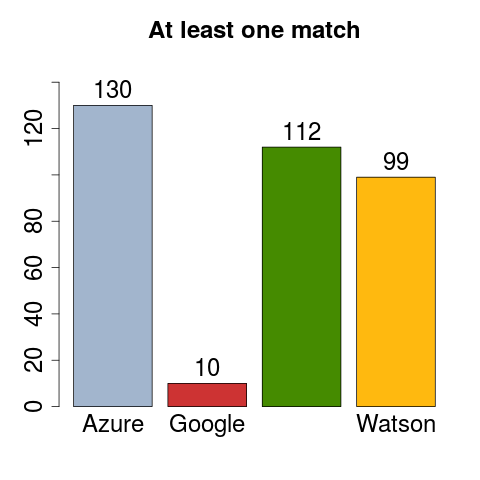
\includegraphics[scale=0.4]{AtLeastOneMatchGraph}
\caption{Histogram of all searches that give back at least one match}
\label{img:testatleastone}
\end{figure}

In Figure~\ref{img:testatleastone} we can see the number of times that services 
gave back at least one correct tag. Even in this case, Azure was the service 
that had the best performance but also Watson and Imagga gave back results that 
are good enough.

\begin{figure}[H]
\centering
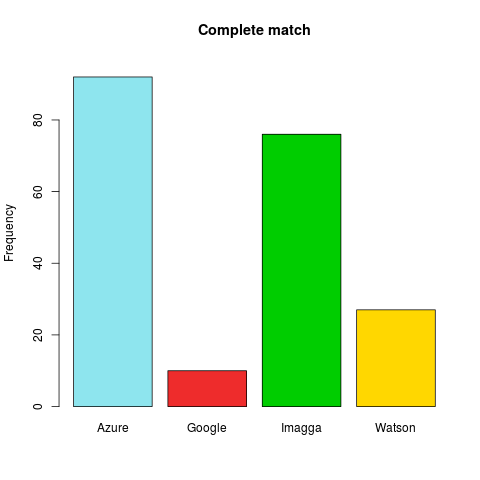
\includegraphics[scale=0.4]{CompleteMatchGraph}
\caption{Histogram of all searches that give back only correct tags}
\label{img:testcompletematch}
\end{figure}

Finally, we present in Figure~\ref{img:testcompletematch} the number of time 
that a service returned a bunch of tags that were all confirmed as matches by a 
user. In this case Azure and Imagga had the best results. In this case even 
Google Reverse Image Search has a positive result, because it gives to the user 
only one tag that could be accepted or not.

\subsection{Character recognition}

\begin{figure}[H]
\centering
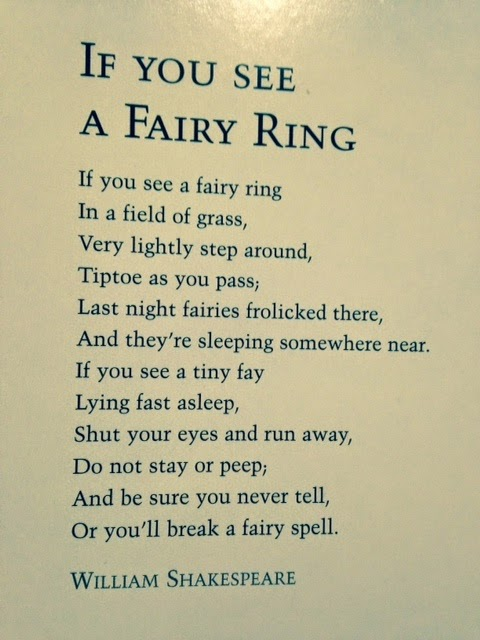
\includegraphics[scale=0.4]{ocr}
\caption{Example of photo with text}
\label{testOCR}
\end{figure}

Execution of OCR in Figure~\ref{testOCR} gives the following result:
\begin{lstlisting}
IF YOU SEE
A FAIRY RING
if you see a fairy ring
in a field of grass,
very lightly step around,
tiptoe as you pass;
last night fairies frolicked there,
and they're sleeping somewhere near.
if you see a tiny fay
lying fast asleep,
shut your eyes and run away,
do not stay or peep;
and be sure you never tell,
or you'll break a fairy spell.
WILLIAM SHAKESPEARE
\end{lstlisting}

In this case, we obtain a perfect match. However, with different resolutions of 
images and different languages, the results are not so good. Unfortunately, we 
were not able to gain data to build a good evaluation set.